\section{Problema 3}

\subsection{Definizione dei sottoproblemi}

Nella risoluzione del problema, abbiamo focalizzato il nostro ragionamento sulla proprietà fondamentale che deve avere un albero per
essere accettabile, ovvero:
\begin{itemize}
    \item Il costo complessivo dell'albero deve essere minimo.
    \item Ogni nodo interno deve avere esattamente due figli.
    \item L'albero ha  esattamente $n$ foglie.
\end{itemize}

\begin{center}
    \textbf{$OPT[i, j]$ rappresenta l'albero di costo minimo contenente le foglie $\{C[j], C[j + 1], ..., C[j + i - 1]\}$ date in input, 
    $\forall i\ \in\ \{1, ..., n\} \land \forall j\ \in\ \{1, ..., n - i + 1\}$ dove $i$ indica la $i-esima$ riga e $j$ indica la $j-esima$ colonna della matrice $OPT$.}
\end{center}

\subsection{Combinazione dei sottoproblemi}

Nel processo di combinazione dei sottoproblemi, abbiamo tenuto presente che un albero ottimale deve essere strutturato in modo binario, cioè deve avere due 
sottoalberi per ogni nodo interno. Questa considerazione ci ha portato a distinguere le foglie in due gruppi: le "foglie destre", che appartengono al sottoalbero 
destro, e le "foglie sinistre", che appartengono al sottoalbero sinistro.

Una volta effettuata questa suddivisione tra sottoalbero destro e sottoalbero sinistro, ci siamo resi conto che la chiave per trovare il valore dell'albero 
ottimale consiste nel provare tutte le possibili suddivisioni fra foglie destre e sinistre e trovare quella con il costo complessivo minimo. Questo si riduce a 
cercare un indice $k$ nell'intervallo $[1 : i - 1]$ tale che il nodo risultante dalla combinazione del sottoalbero sinistro contenente le foglie da $i$ a $i+k$ e del 
sottoalbero destro contenente le foglie da $i+k+1$ a $i+j-1$ sia il più piccolo possibile in termini di costo.

\subsection{Struttura dati}


$$
C = [4, 2, 7]
$$

\begin{enumerate*}[label={}]
    \item {
  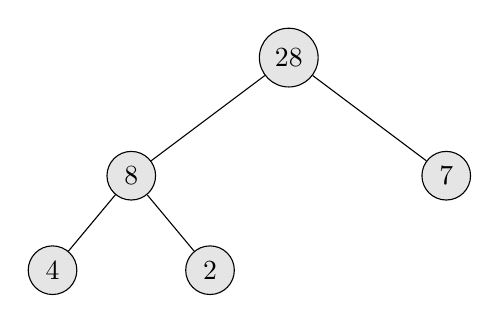
\begin{tikzpicture}[
      level/.style={sibling distance=40mm/#1},
      every node/.style={circle, draw, fill=black!10},
      level 1/.style={level distance=15mm},
      level 2/.style={level distance=12mm},
      level 3/.style={level distance=10mm}
    ]
    \node {28}
    child {node {8}
        child {node {4}}
        child {node {2}}
      }
    child {node {7}};
  \end{tikzpicture}
  }
  \item{
    In questo caso il nostro $k = 0$
  }
\end{enumerate*}


\begin{enumerate*}[label={}]
    \item {
  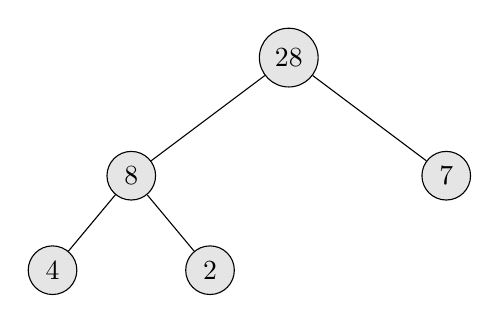
\begin{tikzpicture}[
      level/.style={sibling distance=40mm/#1},
      every node/.style={circle, draw, fill=black!10},
      level 1/.style={level distance=15mm},
      level 2/.style={level distance=12mm},
      level 3/.style={level distance=10mm}
    ]
    \node {28}
    child {node {8}
        child {node {4}}
        child {node {2}}
      }
    child {node {7}};
  \end{tikzpicture}
  }
  \item{
    In questo caso il nostro $k = 1$
  }
\end{enumerate*}
